\section{Code Documentation}
	During the development of RaceTrack it was seen to pay close attention to the concepts of Clean Code (See PDF \textit{PROG1 Clean-Code-Regeln}). All public methods and attributes have also been noted with JavaDoc comments, while private methods and attributes have been commented if deemed necessary.
	The most recent JavaDoc of RaceTrack can be found at the GitHub repository (\url{https://github.zhaw.ch/PathFinder/PSIT3-FS20-IT18ta_WIN-Team5}) under the section \textit{Documentation}.
	\begin{figure}[H]
		\centering
		
\includegraphics[height=2cm,keepaspectratio,center]{img/Implementation_Code-Documentation_Documentation-Section.png}
		\caption{Documentation section in the GitHub repository}
	\end{figure}
	\begin{figure}[H]
		\centering
		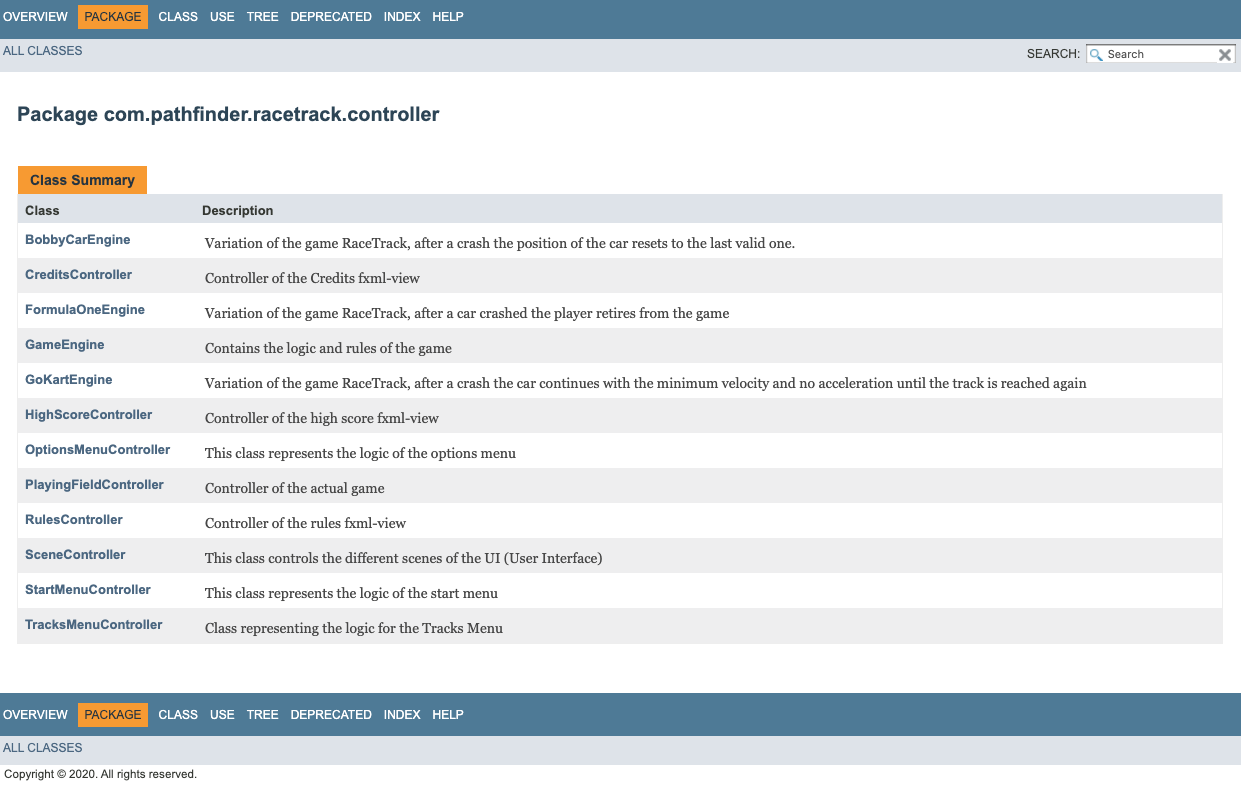
\includegraphics[width=16cm,keepaspectratio,center]{img/Implementation_Code-Documentation_JavaDoc-Example.png}
		\caption{JavaDoc extract of RaceTrack}
	\end{figure}